\documentclass[11pt]{article}

\usepackage{amsmath}
\usepackage{graphicx}
\usepackage{hyperref}
\usepackage{geometry}
\usepackage{float}
\geometry{a4paper, margin=1in}

\title{Project Work: Different Domain Randomization technique for an Hopper Environment}
\author{Luca Ianniello}
\date{\today}

\begin{document}

\maketitle

\begin{abstract}

    This report presents the methodologies and results of the project work done during the Robot Learning course at the University of Turin. The primary objective of the project was to implement a Reinforcement Learning (RL) pipeline for the Hopper environment in OpenAI Gym, utilizing the Soft Actor-Critic (SAC) and Proximal Policy Optimization (PPO) algorithms. Additionally, the project explored the application of Uniform Domain Randomization (UDR). As extension part of the project I decided to explore various domain randomization techniques and their combinations.

    The primary goal of the project is to evaluate the performance of different domain randomization strategies and compare their effectiveness against UDR. The report is structured as follows: the \textit{Introduction} presents the problem and the research goals; the \textit{Related Work} section discusses key contributions in the fields of RL and domain randomization; the \textit{Methodology} outlines the techniques and approaches employed in the study; the \textit{Experiments and Results} section describes the experimental setup and protocols and the analysis of the obtained results; and the \textit{Conclusion} summarizes the outcomes and highlights potential future directions.
    
\end{abstract}

\section{Introduction}

Reinforcement Learning (RL) has emerged as a powerful paradigm for training agents to perform complex tasks in a variety of domains, including robotics, gaming, and natural language processing \cite{Sutton2018}. RL algorithms learn to make decisions by interacting with an environment and receiving feedback in the form of rewards or penalties. By optimizing their policies based on this feedback, RL agents can learn to perform tasks that are difficult to program explicitly \cite{Kober2013}. 

One of the key challenges in RL is the generalization of learned policies to new environments or scenarios. RL models are often trained in simulation environments that may differ significantly from the real-world settings in which they are intended to operate. This discrepancy can lead to a phenomenon known as reality gap, where models fail to transfer their learned behaviors to the real world due to differences in the environment dynamics, sensor noise, or other factors \cite{Kormushev2013, Hofer2020}.

Domain randomization is a technique that aims to bridge the reality gap by training RL models on a diverse set of simulated environments that capture a wide range of possible scenarios. By randomizing the parameters of the simulation, such as physical properties, domain randomization can help models learn robust policies that generalize across different environments \cite{Tobin2017, Peng2018}.

In this project, we explore the impact of different domain randomization techniques on the performance of RL models in the Hopper environment in OpenAI Gym. We focus on the Soft Actor-Critic (SAC) and Proximal Policy Optimization (PPO) algorithms, which are state-of-the-art RL methods that have been shown to achieve strong performance on a variety of tasks \cite{Haarnoja2018, Schulman2017}. We compare the effectiveness of Uniform Domain Randomization (UDR) with other domain randomization strategies, developed as part of the project. 

The primary research goal of this project is to evaluate the performance of different domain randomization techniques and assess their impact on the robustness and generalization of RL models. By conducting a comparative analysis of these methods, we aim to identify the most effective strategies for training agents that can transfer their learned behaviors to new environments.

\section{Related Work}

\subsection{A. Simulation-to-Real Transfer in Robotics}

The problem of sim-to-real transfer in robotics has been a topic of significant interest in recent years, as researchers seek to develop RL models that can operate in real-world settings. Domain randomization has emerged as a promising approach for addressing the reality gap and enabling the transfer of learned policies from simulation to the real world \cite{Peng2018}.

One of the key challenges in sim-to-real transfer is the domain gap between the simulated and real-world environments. By randomizing the parameters of the simulation, such as lighting conditions, object textures, or physical properties, domain randomization can help models learn policies that are robust to these differences \cite{Tobin2017}.

Recent work has explored various domain randomization techniques for sim-to-real transfer, including dynamics randomization. These methods have been shown to improve the generalization and robustness of RL models, enabling them to perform tasks in real-world settings that were previously infeasible \cite{Peng2018}.

In the context of robotics, domain randomization has been applied to a wide range of tasks, including robotic manipulation, locomotion, and navigation. By training agents in diverse simulated environments, researchers have been able to develop RL models that can adapt to changes in the environment dynamics and sensor noise, making them more robust and generalizable \cite{Kormushev2013, Hofer2020}.

The results of these studies have demonstrated the effectiveness of domain randomization for sim-to-real transfer in robotics. By comparing the performance of different domain randomization techniques, researchers can gain insights into the most effective strategies for training agents that can operate in real-world settings.

\subsection{B. Soft Actor-Critic and Proximal Policy Optimization}

Soft Actor-Critic (SAC) and Proximal Policy Optimization (PPO) are two popular RL algorithms that have been shown to achieve strong performance on a variety of tasks. 

SAC is an off-policy RL algorithm that optimizes the policy using a maximum entropy objective, which encourages exploration and improves the robustness of the learned policy. SAC has been shown to achieve state-of-the-art performance on a range of continuous control tasks, including robotic manipulation and locomotion \cite{Haarnoja2018}.

SAC works by learning a stochastic policy that maximizes the expected return while also maximizing the entropy of the policy. This encourages the agent to explore the environment and learn a diverse set of behaviors, which can improve the robustness and generalization of the learned policy.

PPO is an on-policy RL algorithm that optimizes the policy using a clipped surrogate objective, which helps to stabilize training and prevent large policy updates. PPO has been shown to achieve strong performance on a variety of tasks, including robotic manipulation and locomotion \cite{Schulman2017}.

PPO works by learning a deterministic policy that maximizes the expected return while also constraining the policy updates to be within a certain range. This helps to prevent large policy updates that can destabilize training and lead to poor performance.

Both SAC and PPO are well-suited for training agents in complex environments with high-dimensional action spaces, such as the Hopper environment in OpenAI Gym. By comparing the performance of these algorithms with different domain randomization techniques, we can gain insights into the effectiveness of these methods for training robust and generalizable RL models.

\subsection{C. Uniform Domain Randomization}

Uniform Domain Randomization (UDR) is a common domain randomization technique that involves randomizing the parameters of the simulation uniformly across a predefined range. UDR has been shown to improve the generalization and robustness of RL models by exposing them to a diverse set of environments during training \cite{Tobin2017}.

UDR works by sampling random values for the parameters of the simulation, such as lighting conditions, object textures, or physical properties, from a uniform distribution. By training agents on a wide range of simulated environments, UDR can help models learn policies that are robust to changes in the environment dynamics and sensor noise.

While UDR is a simple and effective domain randomization technique, it may not capture the full range of possible scenarios that an agent may encounter in the real world. By exploring more advanced domain randomization strategies, we can potentially improve the generalization and robustness of RL models and enable them to transfer their learned behaviors to new environments more effectively. 

Uniform Domain Randomization is only one of the implemented domain randomization techniques. However, the other implemented algorithms takes inspiration from UDR and tries to improve it by adding more randomness to the simulation.

\section{Methodology}

\subsection{The Hopper Environment}
The techniques and approaches employed in the project are done on the Hopper environment in OpenAI Gym. 
The Hopper Environment is a 2D physics-based environment where the agent controls a 2D hopper to move forward. The agent receives a reward proportional to the distance it moves forward. The goal of the agent is to learn a policy that maximizes the cumulative reward over time. The Hopper environment is challenging due to its high-dimensional action space and complex dynamics, making it an ideal testbed for evaluating the performance of RL algorithms. 
The state space is continual and it is composed by the positional values of different body parts. In details, the state space is composed by the following values:
\begin{itemize}
    \item Z-coordinate of the top, so the height of the hopper
    \item Angle of the top
    \item Angle of the thigh joint
    \item Angle of the leg joint
    \item Angle of the foot joint
    \item Velocity of the x-coordinate of the top
    \item Velocity of the z-coordinate of the top
    \item Angular velocity of the top
    \item Angular velocity of the thigh joint
    \item Angular velocity of the leg joint
    \item Angular velocity of the foot joint
\end{itemize}

The action space is also continuous and it is composed by the following values:
\begin{itemize}
    \item Torque applied to the thigh joint
    \item Torque applied to the leg joint
    \item Torque applied to the foot joint
\end{itemize}

One important aspect of the Hopper environment is related to the masses of the body parts. These masses are handled in the vector body-masses of the model and in details this vector is composed by the following values:
\begin{itemize}
    \item Mass of the world
    \item Mass of the torse
    \item Mass of the thigh
    \item Mass of the leg
    \item Mass of the foot
\end{itemize}

In our Hopper Environment, we consider the torse mass fixed as the original values less 1.0 in the source domain and we will not modify the mass of the world. The mass of the thigh, leg and foot will be modified by the domain randomization techniques.

The common Reinforcement Learning pipeline was done using the Soft Actor-Critic (SAC) and Proximal Policy Optimization (PPO) algorithms. In the experimental section, we will compare the performance of these two algorithms considering the different domain randomization techniques.


\subsection{Soft Actor-Critic (SAC) and Proximal Policy Optimization (PPO)}

In this experiments, the Soft Actor-Critic (SAC) and Proximal Policy Optimization (PPO) algorithms were used as implemented in the \texttt{stable-baselines3} library. These two reinforcement learning algorithms differ significantly in their nature: SAC is an off-policy algorithm, whereas PPO is an on-policy algorithm. Their diversity brings to some adjustments to the training process, particularly when incorporating domain randomization techniques.

For the PPO algorithm, a \texttt{batch\_size} variable was defined to ensure consistency in training. This variable was set equal to the number of steps (\texttt{n\_steps}) of the PPO model. This design choice aligns with the requirements of on-policy algorithms, which rely on collecting batches of transitions from the same policy before performing updates. By ensuring that domain randomization parameters remain fixed during the collection of transitions within each batch, the PPO algorithm was able to compute accurate advantage estimates and perform stable updates to the policy.

In contrast, SAC, due to its nature of off-policy algorithm, does not require such synchronization. Randomization was applied at every step without affecting the training stability, as SAC uses a replay buffer and updates the policy based on previously collected transitions rather than requiring consistency within a single batch of collected experiences.

\subsection{Domain Randomization Techniques}

The first type of implemented domain adaptation technique is the Uniform Domain Randomization (UDR). This technique is the simplest one and it is done by sampling the mass of the thigh, leg and foot from a uniform distribution. Instead of using a common range composed by a lower and an upper bound, I have defined three categories, one for each body mass. The reason behind this choice is to have a more controlled randomization of the masses. The standard original values of the masses are different  for each body part. In details, the original values of the body mass in our custom hopper environment are:
\begin{itemize}
    \item Mass of the thigh: 3.92699082
    \item Mass of the leg: 2.71433605
    \item Mass of the foot: 5.0893801
\end{itemize}

The ranges of the masses are defined considering the original values of the masses and create a range of values around the original values, considering as lower bound the original value less 0.2 and as upper bound the original value plus 0.2. The reason behind this choice is the consequence of different test done with SAC and PPO algorithm on ranges of larger values. In the experiment section, I have tested also large ranges (0.8 and 1.5).  In this tests, the agent was not able to learn a good policy in both the algorithms. Larger ranges introduce more diverse physical behaviors, making it harder for the policy to generalize across all possible configurations. Both SAC and PPO rely on exploration to find optimal actions. If the environment is too diverse, the agent may struggle to identify patterns that consistently lead to high rewards.\\

The second type of implemented domain randomization technique is based on the idea of starting with large ranges and reducing them as training progresses. The name associated with this algorithm is Reducing Ranged Domain Randomization (RRDR). This method calculates a dynamic factor, referred to as the RRDR factor, which decreases over time to progressively narrow the randomization ranges. At the start of training, large ranges are used to encourage exploration of diverse dynamics. The range expansion is applied only to the upper bound, while the lower bound remains fixed. These ranges are defined around the original masses of the thigh, leg, and foot, with initial bounds expanded by the RRDR factor. The RRDR factor is determined based on the current training progress: during the first 20\% of the total timesteps, large ranges are used with an upper-bound increment of 0.5. Following this phase, a logarithmic reduction is applied to the RRDR factor until 80\% of the total timesteps is reached. After this point, the increment becomes 0, and the ranges converge to those used in Uniform Domain Randomization (UDR). The mass for each body part is then sampled from a normal distribution, where the mean shifts toward the original mass values as training progresses, and the standard deviation decreases to focus the sampling range. This approach ensures that the agent is exposed to a wide variety of dynamics initially, while gradually narrowing the range toward the target domain, facilitating both exploration and fine-tuning during different phases of training.\\

The third type of implemented domain randomization technique is called Incremental Ranges Expansion Domain Randomization (IRE). This method focuses on gradually increasing the randomization ranges as training progresses, allowing the agent to adapt initially to a narrower, more controlled range before being exposed to more diverse dynamics. The algorithm begins with ranges defined around the original masses of the thigh, leg, and foot, equal to the ones used in the UDR. The lower bound of the range remains fixed, while the upper bound is incrementally expanded. The expansion of the ranges is determined dynamically based on the training progress. Specifically, the upper bound of each range increases logarithmically with training progress, scaled by a factor of 0.5 to control the expansion rate. In this way, at the end of the training progress, the ranges are equal to the starting ranges of RRDR. This gradual increase ensures a smooth transition from focused exploration at the start of training to a broader exploration of dynamics as training continues. For each body part, the mass is sampled from a normal distribution centered on the midpoint of the dynamically adjusted range, and the standard deviation of the distribution decreases as training progresses, focusing the sampling around the mean. This approach is inspired by the principles of curriculum learning, where tasks or training examples are presented in a structured manner, starting with simpler scenarios and progressively increasing complexity. This behaviour is partially described in the Automatic Domain Randomization approach \cite{Akkaya2020}. In the context of IRE, the early training phases expose the agent to predictable dynamics within narrower ranges, facilitating stable policy learning. As training progresses, the broader ranges introduce more diverse dynamics, improving the agent's robustness and generalization to varying conditions. By the end of training, the agent is exposed to a wide range of dynamics, promoting adaptability and performance across different scenarios.\\

The next three domain randomization techniques are based on the use of the previous three algorithm in different orders.\\

The fourth type of implemented domain randomization technique is called Exploration Uniform Domain Randomization (EUDR). This method divides the training process into three distinct phases, each focusing on a specific goal: exploration, controlled randomization, and exploitation. The phases are determined by dividing the total training steps into three parts: an increment phase, where the IRE algorithm is executed, a reducing phase, where the RRDR algorithm is executed, and a uniform phase, where the UDR algorithm is executed. During the increment phase, the algorithm focuses on exploration by gradually increasing the randomization ranges around the original mass values. This phase uses a higher entropy coefficient for the policy to encourage exploration. Next, in the reducing phase, the randomization ranges are progressively narrowed, allowing the agent to explore more diverse dynamics while maintaining a controlled focus. The entropy coefficient is reduced during this phase to stabilize policy learning. Finally, the uniform phase applies fixed randomization ranges that align with the original Uniform Domain Randomization (UDR) approach. This phase uses the smallest entropy coefficient, emphasizing exploitation of the learned policy. The incremented and reduced ranges are perfectly alligned, considering the values previously indicated. The choice of entropy coefficients is dynamically adjusted based on the reinforcement learning algorithm being used. For instance, higher entropy coefficients are set for the Soft Actor-Critic (SAC) algorithm during the early exploration phase, while the Proximal Policy Optimization (PPO) algorithm uses smaller coefficients to balance exploration and exploitation. The algorithm dynamically determines the current phase and adjusts both the entropy coefficients and randomization ranges accordingly.\\

The fifth domain randomization technique implemented is the Dynamic Range Cycle Domain Randomization (DRC). This method divides the training process into three recurring phases: Uniform Domain Randomization, Incremental Ranges Expansion Domain Randomization, and Reducing Ranged Domain Randomization. The algorithm cycles through these phases with the aim of balancing exploration and exploitation at different stages of training. Initially, the uniform phase applies fixed randomization ranges around the original masses, promoting a balanced exploration of the dynamics. This phase is followed by the increment phase, where the randomization ranges are progressively expanded. The larger ranges in this phase encourage exploration of diverse dynamics beyond the original environment parameters. The final phase, reducing randomization, narrows the ranges incrementally, allowing the agent to focus on mastering dynamics closer to the target domain.The DRC algorithm dynamically adjusts the entropy coefficient based on the reinforcement learning algorithm in use, such as Soft Actor-Critic (SAC) or Proximal Policy Optimization (PPO). During the increment phase, the entropy coefficient is increased to enhance exploration, while it is reduced during the uniform and reducing phases to stabilize learning and prioritize exploitation. The phases are proportionally divided across the total training steps, with 20\% of the steps allocated to the uniform phase, 40\% to the increment phase, and 40\% to the reducing phase. This cyclic structure ensures that the agent is exposed to diverse dynamics at regular intervals, facilitating both robust exploration and targeted fine-tuning. By combining adaptive range management and entropy tuning, DRC provides a structured yet flexible framework for training agents in complex environments. A similar approach was used in \cite{Akkaya2020}. The defined Automatic Domain Randomization, however, increases and reduces the distribution thresholds considering the obtained average model performance, while in my case, the distribution is increased and reduced considering the training steps.\\

The sixth and last domain randomization method implemented is the Dynamic Exploration Domain Randomization (DEDR). This technique divides the training process into three phases: Reducing Ranged Domain Randomization, Uniform Domain Randomization, and Incremental Ranges Expansion Domain Randomization, each designed to guide the agent through distinct exploration and exploitation strategies during training. Initially, the reducing phase employs large randomization ranges around the original masses, encouraging extensive exploration of the environment's dynamics. This phase, which spans 40\% of the total training steps, ensures that the agent is exposed to diverse variations early in the training process, helping to prevent premature convergence to suboptimal policies. The reducing phase transitions into the uniform phase, accounting for 30\% of the training steps, where fixed randomization ranges are applied. These ranges are equal to the decreased ranges obtained after the RRDR algorithm end, striking a balance between exploration and stability. In the final increment phase, spanning the remaining 30\% of the training, the randomization ranges are gradually expanded again, focusing the exploration on variations near those encountered during the uniform phase. The entropy coefficient is dynamically adjusted based on the training phase and reinforcement learning algorithm in use. During the reducing phase, the entropy coefficient is set higher to promote exploration, while it is lowered during the uniform phase to stabilize learning. In the increment phase, a moderate entropy coefficient ensures controlled exploration near the learned dynamics. This structured progression of exploration and exploitation phases, combined with adaptive range adjustments, enables the DEDR method to systematically guide the agent toward robust policy learning in dynamic environments.\\

\section{Experiments and Results}

In this section, I present the results obtained using the Soft Actor-Critic (SAC) and Proximal Policy Optimization (PPO) algorithms with various domain randomization techniques. The results are illustrated through the learning curve of the two algorithms, evaluated in both the source and target domains.

For each algorithm and each domain randomization technique, two distinct models were trained: one in the source domain and the other in the target domain. The only difference between the source and the target domain is related to the mass values of the torse. This value is not subject to randomization, but in the source domain the value is 1.0 less than the corresponding value in the target domain. 
The analysis focuses on the mean reward and standard deviation obtained during the evaluation of these models in their respective domains. Additionally, I evaluate the performance of the source-trained model when deployed in the target domain to assess its generalization capabilities. I will consider the results obtained in the target->target evaluation as a upper bound for the performance of the models in the target domain and the results obtained in the source->target evaluation as a lower bound for the performance of the models in the target domain. 

The training phase for each experiment was conducted over 250,000 timesteps, while the evaluation was performed across 100 episodes to ensure statistically significant results, instead of using the indicated 50 test episodes.

\subsection{Without Domain Randomization}

The first set of experiments was conducted without domain randomization, serving as a baseline for comparison with the domain randomization techniques. The following four pictures shows the learning curve of SAC and PPO considering the source and the target domain without domain randomization.

\begin{figure}[H]
    \centering
    \begin{minipage}{0.45\textwidth}
        \centering
        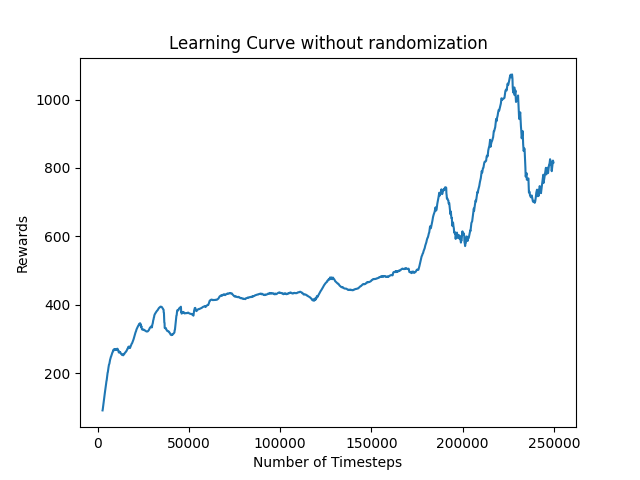
\includegraphics[width=\textwidth]{../images/Learning_Curve_SAC_no_rand_Source.png}
        \caption{SAC Source Domain without DR}
        \label{fig:sac_source_no_dr}
    \end{minipage}
    \hfill
    \begin{minipage}{0.45\textwidth}
        \centering
        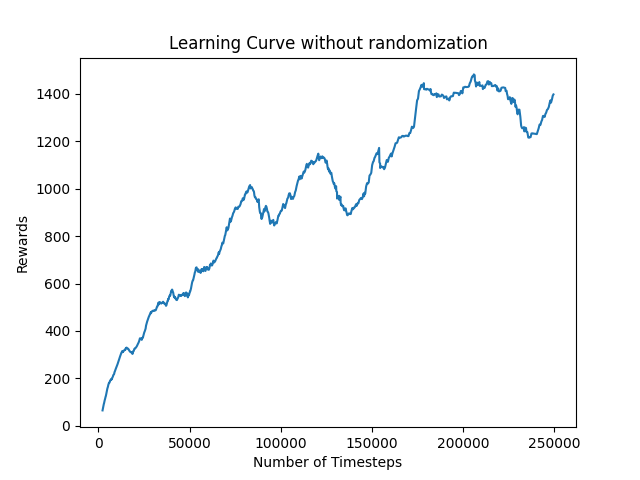
\includegraphics[width=\textwidth]{../images/Learning_Curve_SAC_no_rand_Target.png}
        \caption{SAC Target Domain without DR}
        \label{fig:sac_target_no_dr}
    \end{minipage}
    \vfill
    \begin{minipage}{0.45\textwidth}
        \centering
        \includegraphics[width=\textwidth]{../images/Learning_Curve_PPO_no_rand_Source.png}
        \caption{PPO Source Domain without DR}
        \label{fig:ppo_source_no_dr}
    \end{minipage}
    \hfill
    \begin{minipage}{0.45\textwidth}
        \centering
        \includegraphics[width=\textwidth]{../images/Learning_Curve_PPO_no_rand_Source.png}
        \caption{PPO Target Domain without DR}
        \label{fig:ppo_target_no_dr}
    \end{minipage}
\end{figure}

In the following table, I report the mean reward and standard deviation obtained by the models trained without domain randomization in the source and target domains:

\begin{table}[H]
    \centering
    \begin{tabular}{|l|c|c|c|}
        \hline
        \textbf{Algorithm} & \textbf{Evaluation} & \textbf{Mean Reward} & \textbf{Standard Deviation} \\ \hline
        SAC & Source $\rightarrow$ Source & 1245.45 & 53.04 \\ 
        SAC & Source $\rightarrow$ Target & 1109.39 & 70.13 \\ 
        SAC & Target $\rightarrow$ Target & 1656.45 & 116.75 \\ \hline
        PPO & Source $\rightarrow$ Source & 1319.98 & 229.10 \\ 
        PPO & Source $\rightarrow$ Target & 680.68 & 11.35 \\ 
        PPO & Target $\rightarrow$ Target & 1268.77 & 214.69 \\ \hline
    \end{tabular}
    \caption{Results of SAC and PPO without domain randomization.}
    \label{tab:results_no_randomization}
\end{table}

The results show that both SAC and PPO achieve higher mean rewards in the target domain compared to the source domain when trained without domain randomization. However, the standard deviation of the rewards is higher in the target domain, indicating that the models exhibit greater variability in their performance. The generalization capabilities of the models are also evident, with the source-trained models achieving competitive performance in the target domain for the SAC algorithm. These results suggest that the models are able to adapt to the dynamics of the target domain without the need for domain randomization.

In both cases the PPO algorithm has a lower mean reward and a lower standard deviation compared to the SAC algorithm. This is due to the fact that the PPO algorithm is an on-policy algorithm and it is more stable than the SAC algorithm. The SAC algorithm is an off-policy algorithm and it is more prone to instability during the training process. This is the reason why the SAC algorithm has a higher standard deviation compared to the PPO algorithm. This aspect will be fondamental to understand the impact of the domain randomization techniques on the two algorithms. 

In the source to target evaluation, I obtained the lowest results for both PPO and SAC. This behaviour is expected. This phenomenon is known as domain shift, and it can lead to a mismatch between the training and testing conditions. The model trained in the source domain has learned a policy optimized for the source domain, which may not generalize well to the target domain if there are significant differences in the environment. 

In the evaluation, the main focus is done on the results obtained on the source to target evalutation. As we can see in these results, SAC achieves higher values in the target to target evaluation and also PPO achieves results that are high. However, in real-world settings, training an RL agent directly in the target environment (e.g., physical robots) is often prohibitively expensive. It requires significant computational resources, time, and the risk of damaging physical systems during experimentation. In contrast, simulation allows for faster and cheaper training cycles, reducing the need for costly trial and error in real-world environments. 

The idea of testing different domain randomization techniques is to understand how the agent can learn a policy that can generalize well in the target domain. The results obtained in the source to target evaluation are the most important to understand the impact of the domain randomization techniques on the generalization capabilities of the agent.

\subsection{Uniform Domain Randomization (UDR)}

The next set of experiments was conducted using the Uniform Domain Randomization (UDR) technique. The following four pictures shows the learning curve of SAC and PPO considering the source and the target domain with UDR and ranges defined with an increment of 0.2 (small increment).

\begin{figure}[H]
    \centering
    \begin{minipage}{0.45\textwidth}
        \centering
        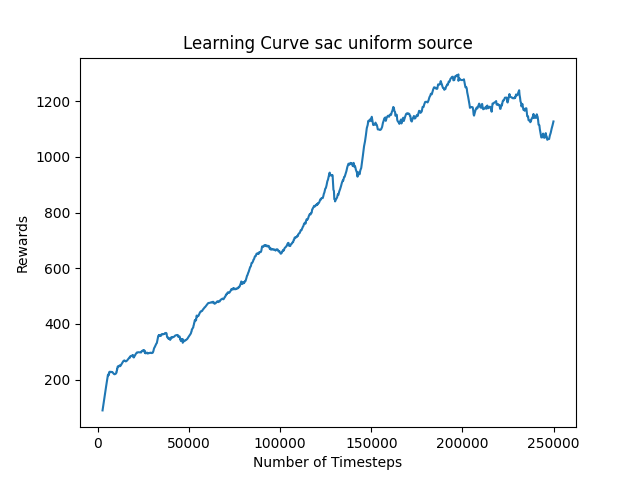
\includegraphics[width=\textwidth]{../images/Learning_Curve_SAC_Uniform_Source.png}
        \caption{SAC Source Domain with UDR }
        \label{fig:sac_source_udr}
    \end{minipage}
    \hfill
    \begin{minipage}{0.45\textwidth}
        \centering
        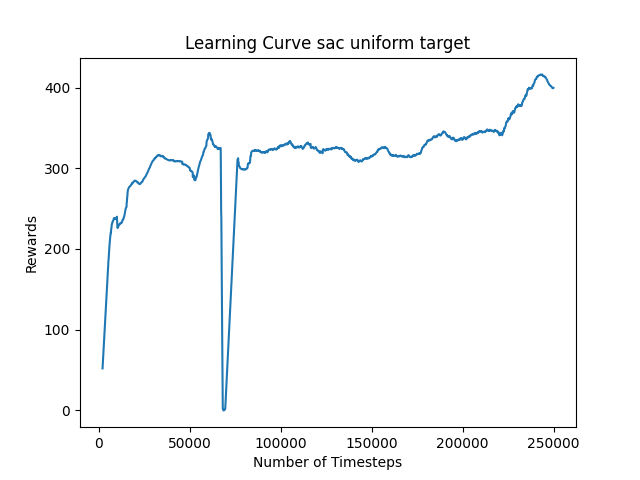
\includegraphics[width=\textwidth]{../images/Learning_Curve_SAC_Uniform_Target.png}
        \caption{SAC Target Domain with UDR}
        \label{fig:sac_target_udr}
    \end{minipage}
    \vfill
    \begin{minipage}{0.45\textwidth}
        \centering
        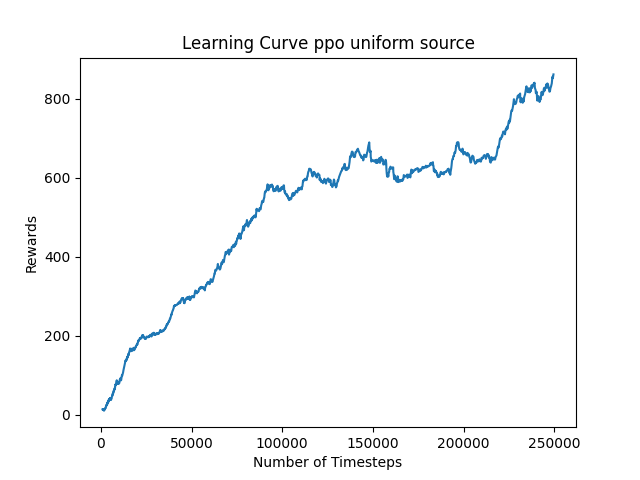
\includegraphics[width=\textwidth]{../images/Learning_Curve_PPO_Uniform_Source.png}
        \caption{PPO Source Domain with UDR}
        \label{fig:ppo_source_udr}
    \end{minipage}
    \hfill
    \begin{minipage}{0.45\textwidth}
        \centering
        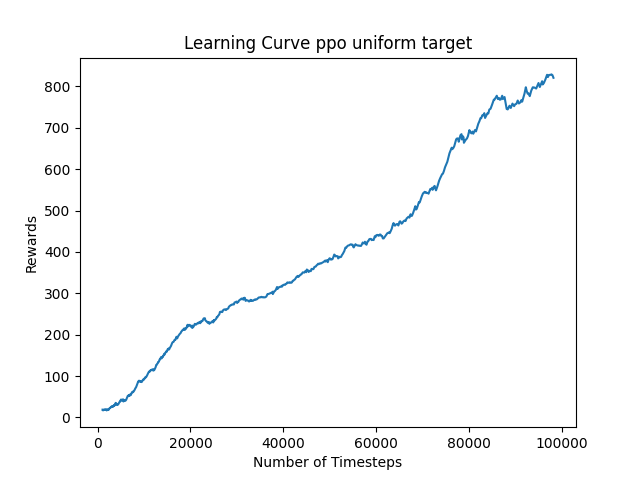
\includegraphics[width=\textwidth]{../images/Learning_Curve_PPO_Uniform_Target.png}
        \caption{PPO Target Domain with UDR}
        \label{fig:ppo_target_udr}
    \end{minipage}
\end{figure}

In the following table, I report the mean reward and standard deviation obtained by the models trained with Uniform Domain Randomization in the source and target domains:

\begin{table}[H]
    \centering
    \begin{tabular}{|l|c|c|c|}
        \hline
        \textbf{Algorithm} & \textbf{Evaluation} & \textbf{Mean Reward} & \textbf{Standard Deviation} \\ \hline
        SAC & Source $\rightarrow$ Source & 871.41 & 45.61 \\ 
        SAC & Source $\rightarrow$ Target & 648.01 & 4.95 \\ 
        SAC & Target $\rightarrow$ Target & 415.55 & 3.49 \\ \hline
        PPO & Source $\rightarrow$ Source & 1408.03 & 43.86 \\ 
        PPO & Source $\rightarrow$ Target & 1388.90 & 191.31 \\ 
        PPO & Target $\rightarrow$ Target & 872.79 & 10.77 \\ \hline
    \end{tabular}
    \caption{Results of SAC and PPO with Uniform Domain Randomization.}
    \label{tab:results_udr}
\end{table}

The results show that both SAC and PPO achieve lower mean rewards in the target domain compared to the source domain when trained with Uniform Domain Randomization. The standard deviation of the rewards is also lower in the target domain, indicating that the models exhibit less variability in their performance. The generalization capabilities of the models are evident in the PPO algorithm, with the source-trained models achieving competitive performance in the target domain. These results suggest that Uniform Domain Randomization can improve the robustness and generalization of the models, enabling them to adapt to different dynamics.

These results suggest that, while SAC excels in stability within its domain, it faces greater challenges when generalizing across domains, especially with domain randomization. PPO, on the other hand, is more robust to domain shifts, demonstrating better generalization across both the source and target domains even with UDR applied. This highlights PPO’s ability to efficiently explore and adapt in more diverse environments. The rendered results shows that PPO was able to find a policy that moves correctly the hopper in both source and target domain, while SAC was not able to find a good policy in the target domain.

The results obtained can be attributed to the use of fixed categories for the mass values, where the ranges are too small. 
The Soft Actor-Critic algorithm, being more sensitive to changes in the environment, struggles to adapt to the target domain, where the torso mass is different from the source domain. SAC’s exploration capabilities are constrained by the small randomization ranges applied to the leg, foot, and thigh masses. This limits the algorithm's ability to explore and learn a robust policy that generalizes well in the target domain, where the torso mass difference plays a larger role.
On the other hand, the Proximal Policy Optimization algorithm, which is on-policy and more stable, handles the torso mass difference better. Due to its stability, PPO is able to learn a policy that generalizes better in the target domain, despite the unrandomized torso mass difference.

The current results with Uniform Domain Randomization are suboptimal for SAC because SAC struggles to explore the environment effectively, largely due to the limited ranges of mass randomization. Expanding the randomization ranges for the leg, foot, and thigh masses could provide SAC with more opportunities to explore and adapt its policy to a broader set of conditions, which may improve generalization across both the source and target domains. 

The next two tests will consider the use of larger ranges for the mass values. The results obtained in these tests will be compared with the results obtained with the small ranges.

First of all, I have defined a medium increment ranges, where ranges are increased of 0.8. The following four pictures shows the learning curve of SAC and PPO considering the source and the target domain with UDR and ranges defined with an increment of 0.8 (medium increment).

\begin{figure}[H]
    \centering
    \begin{minipage}{0.45\textwidth}
        \centering
        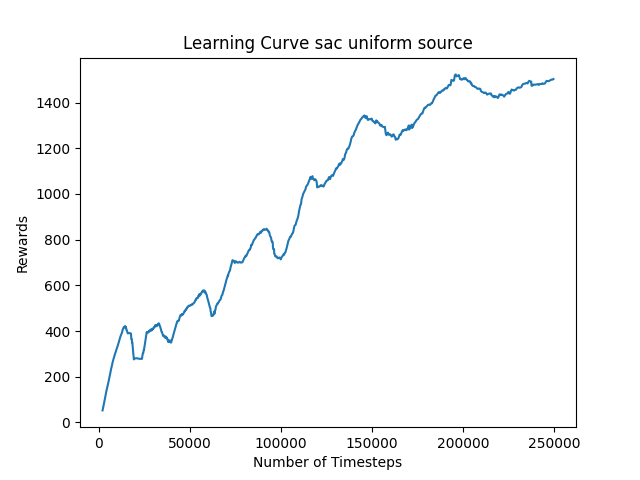
\includegraphics[width=\textwidth]{../images/Learning_Curve_SAC_Uniform_Medium_Source.png}
        \caption{SAC Source Domain with UDR and medium ranges}
        \label{fig:sac_source_udr_medium}
    \end{minipage}
    \hfill
    \begin{minipage}{0.45\textwidth}
        \centering
        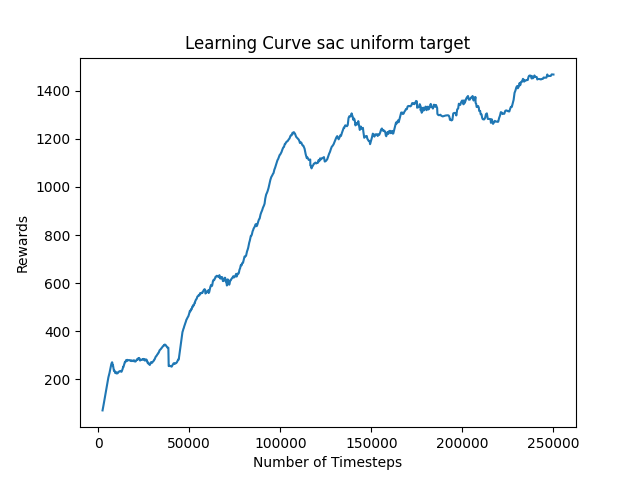
\includegraphics[width=\textwidth]{../images/Learning_Curve_SAC_Uniform_Medium_Target.png}
        \caption{SAC Target Domain with UDR and medium ranges}
        \label{fig:sac_target_udr_medium}
    \end{minipage}
    \vfill
    \begin{minipage}{0.45\textwidth}
        \centering
        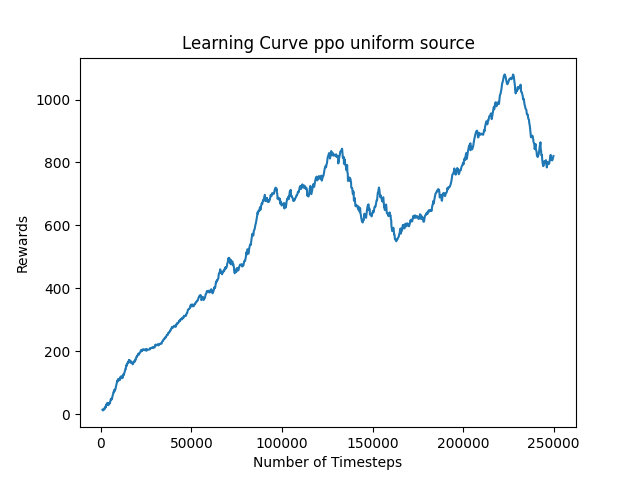
\includegraphics[width=\textwidth]{../images/Learning_Curve_PPO_Uniform_Medium_Source.png}
        \caption{PPO Source Domain with UDR and medium ranges}
        \label{fig:ppo_source_udr_medium}
    \end{minipage}
    \hfill
    \begin{minipage}{0.45\textwidth}
        \centering
        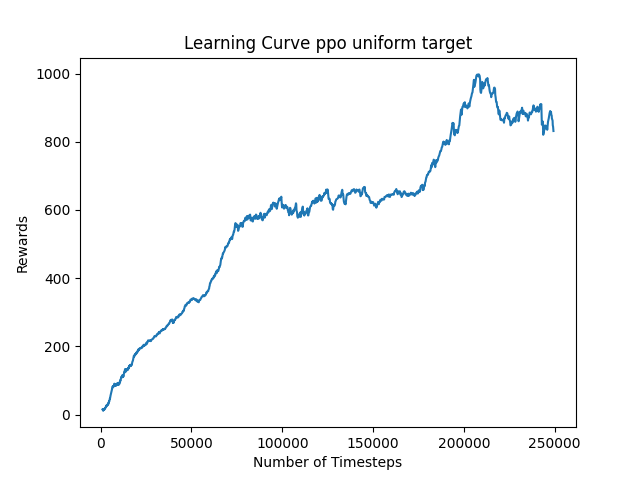
\includegraphics[width=\textwidth]{../images/Learning_Curve_PPO_Uniform_Medium_Target.png}
        \caption{Figure 12. PPO Target Domain with UDR and medium ranges}
        \label{fig:ppo_target_udr_medium}
    \end{minipage}
\end{figure}

In the following table, I report the mean reward and standard deviation obtained by the models trained with Uniform Domain Randomization and larger ranges in the source and target domains:

\begin{table}[H]
    \centering
    \begin{tabular}{|l|c|c|c|}
        \hline
        \textbf{Algorithm} & \textbf{Evaluation} & \textbf{Mean Reward} & \textbf{Standard Deviation} \\ \hline
        SAC & Source $\rightarrow$ Source & 1557.56 & 18.36 \\ 
        SAC & Source $\rightarrow$ Target & 1459.58 & 142.15 \\ 
        SAC & Target $\rightarrow$ Target & 1463.26 & 2.08 \\ \hline
        PPO & Source $\rightarrow$ Source & 935.47 & 82.87 \\ 
        PPO & Source $\rightarrow$ Target & 746.77 & 51.19 \\ 
        PPO & Target $\rightarrow$ Target & 1048.83 & 248.37 \\ \hline
    \end{tabular}
    \caption{Results of SAC and PPO with Uniform Domain Randomization and medium ranges.}
    \label{tab:results_udr_medium}
\end{table}

The results show an increment of the mean reward values of the SAC model, but an decreasing of the mean reward values of the PPO model, comparing them with the results obtained in the previous UDR analysis. The rendering of the results shows that the SAC model is not able to find a good policy that moves correctly the hopper in both the source and the target domain, even there is an improvemenent compared to previous results. However, the results obtained with PPO shows that the model is not able to find a good policy to move correctly the hopper in both the environments. 

The following four pictures shows the learning curve of SAC and PPO considering the source and the target domain with UDR and ranges defined with an increment of 1.5 (large increment).

\begin{figure}[H]
    \centering
    \begin{minipage}{0.45\textwidth}
        \centering
        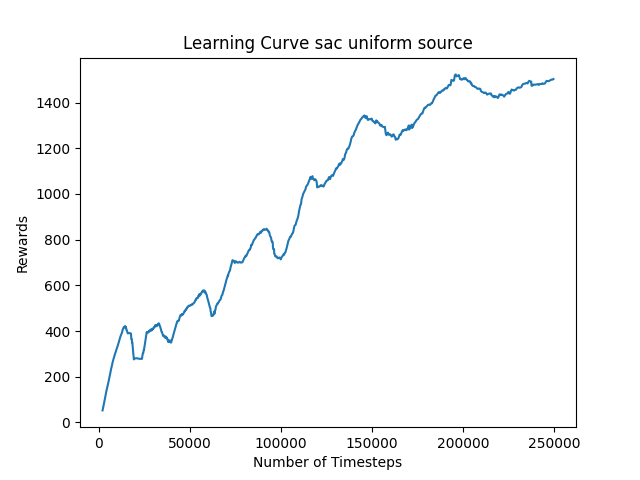
\includegraphics[width=\textwidth]{../images/Learning_Curve_SAC_Uniform_Large_Source.png}
        \caption{SAC Source Domain with UDR and larger ranges}
        \label{fig:sac_source_udr_larger}
    \end{minipage}
    \hfill
    \begin{minipage}{0.45\textwidth}
        \centering
        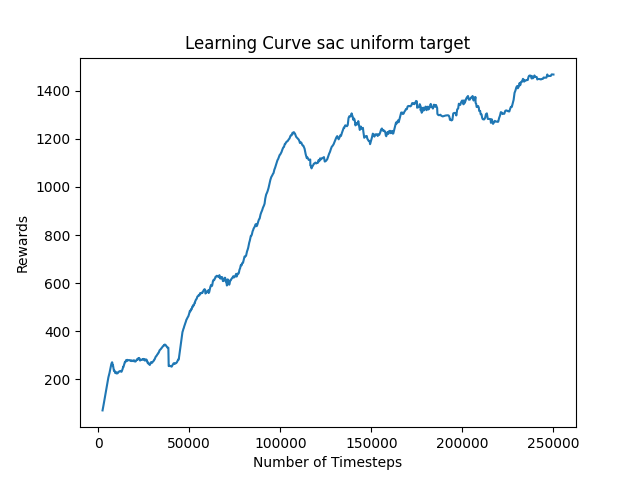
\includegraphics[width=\textwidth]{../images/Learning_Curve_SAC_Uniform_Large_Target.png}
        \caption{SAC Target Domain with UDR and larger ranges}
        \label{fig:sac_target_udr_larger}
    \end{minipage}
    \vfill
    \begin{minipage}{0.45\textwidth}
        \centering
        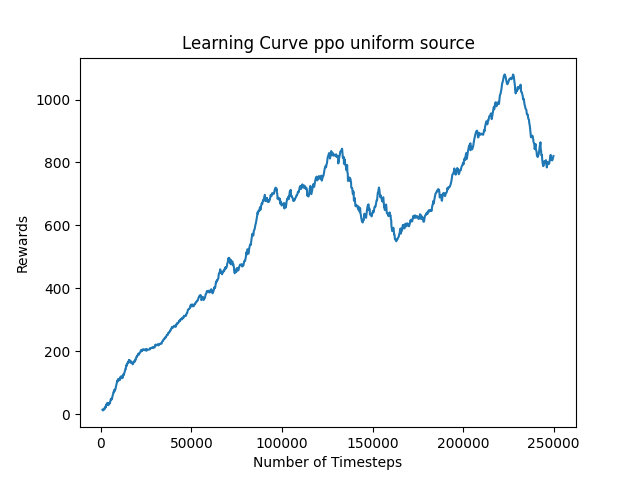
\includegraphics[width=\textwidth]{../images/Learning_Curve_PPO_Uniform_Large_Source.png}
        \caption{PPO Source Domain with UDR and larger ranges}
        \label{fig:ppo_source_udr_larger}
    \end{minipage}
    \hfill
    \begin{minipage}{0.45\textwidth}
        \centering
        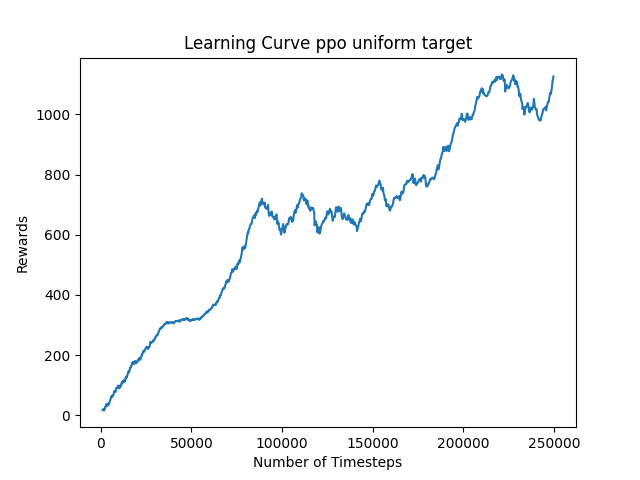
\includegraphics[width=\textwidth]{../images/Learning_Curve_PPO_Uniform_Large_Target.png}
        \caption{PPO Target Domain with UDR and larger ranges}
        \label{fig:ppo_target_udr_larger}
    \end{minipage}
\end{figure}

In the following table, I report the mean reward and standard deviation obtained by the models trained with Uniform Domain Randomization and larger ranges in the source and target domains:

\begin{table}[H]
    \centering
    \begin{tabular}{|l|c|c|c|}
        \hline
        \textbf{Algorithm} & \textbf{Evaluation} & \textbf{Mean Reward} & \textbf{Standard Deviation} \\ \hline
        SAC & Source $\rightarrow$ Source & 718.15 & 66.19 \\ 
        SAC & Source $\rightarrow$ Target & 735.93 & 44.44 \\ 
        SAC & Target $\rightarrow$ Target & 1176.75 & 273.61 \\ \hline
        PPO & Source $\rightarrow$ Source & 811.97 & 70.98 \\ 
        PPO & Source $\rightarrow$ Target & 1086.12 & 57.55 \\ 
        PPO & Target $\rightarrow$ Target & 1502.40 & 35.66 \\ \hline
    \end{tabular}
    \caption{Results of SAC and PPO with Uniform Domain Randomization and larger ranges.}
    \label{tab:results_udr_larger}
\end{table}

The results show that the mean reward values of the SAC model are lower than the mean reward values obtained with the medium ranges, while the once obtained with PPO are higher. However, The rendering of the results shows that both the SAC model and the PPO model are not able to find a good policy that moves correctly the hopper in both the source and the target domain. The results obtained with the PPO model are higher than the results obtained with the medium ranges. 

The larger ranges in the Uniform Domain Randomization approach provide more opportunities for exploration and adaptation, allowing the agent to experience a wider range of dynamics and environments. This can help the agent learn more robust policies that generalize well across domains, improving adaptability and performance. However, the larger ranges can also introduce more variability and instability in learning, making it difficult for the agent to converge on a good solution. This is reflected in the higher standard deviation in the results, where the agent might learn to adapt to randomization but with less stability, especially when trained with a large variety of parameter settings. This limitation highlights the need for more adaptive domain randomization techniques that can provide a balance between exploration and exploitation, allowing the agent to adapt to a wide range of dynamics while maintaining robustness and generalization capabilities.

The choice of using lower ranges can be a good choice because with small ranges I have obtained good results with PPO, considering a lower computational time, considering the lower results obtained with large ranges with SAC, considering an higher computational time.

From these results, we can conclude that UDR helps PPO maintain better performance when transitioning to the target domain, as evidenced by the relatively higher rewards and the smaller drop in performance from the source to the target domain. For SAC, UDR doesn't seem to fully compensate for the torso mass shift, leading to lower performance in the target domain.

In general, while UDR allows the models to adapt to the target domain, the use of fixed ranges for values can cause overfitting to the source domain. The models may learn a policy that is too specific to the source domain, making it difficult to generalize to the target domain. In addition, while UDR helps the agent to handle different configurations and environmental shifts, the variability introduced during training could lead to instability in learning. This is reflected in the higher standard deviation in PPO’s "source to target" results, where the model might learn to adapt to randomization but with less stability, especially when trained with a large variety of parameter settings. This limitation highlights the need for more adaptive domain randomization techniques that can provide a balance between exploration and exploitation, allowing the models to adapt to a wide range of dynamics while maintaining robustness and generalization capabilities.

\subsection{Reducing Ranged Domain Randomization (RRDR)}

The next set of experiments was conducted using the Reducing Ranged Domain Randomization (RRDR) technique. The following four pictures shows the learning curve of SAC and PPO considering the source and the target domain with RRDR.

\begin{figure}[H]
    \centering
    \begin{minipage}{0.45\textwidth}
        \centering
        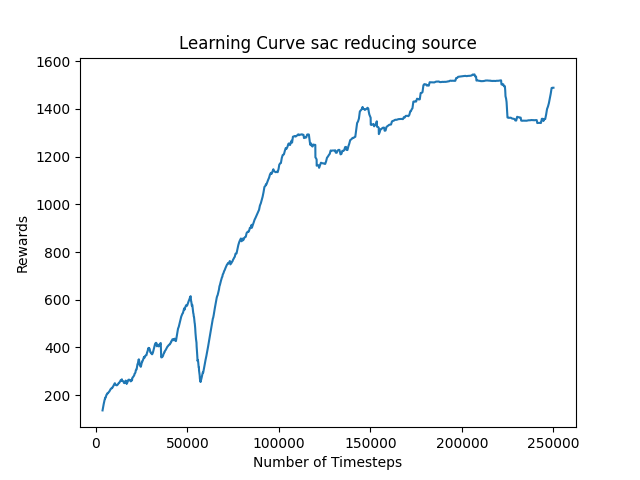
\includegraphics[width=\textwidth]{../images/Learning_Curve_SAC_Reducing_Source.png}
        \caption{SAC Source Domain with RRDR}
        \label{fig:sac_source_rrdr}
    \end{minipage}
    \hfill
    \begin{minipage}{0.45\textwidth}
        \centering
        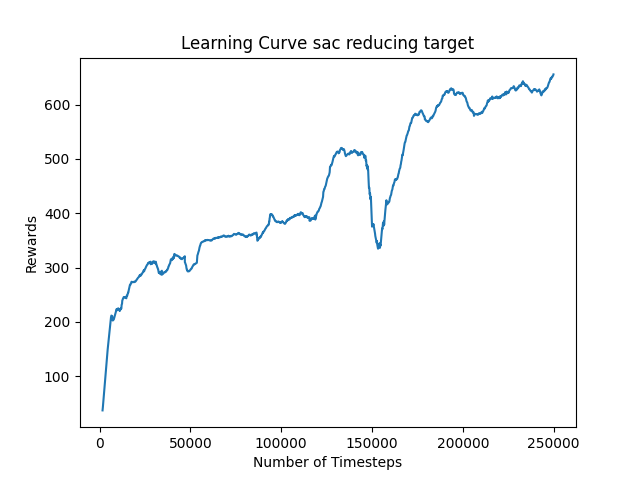
\includegraphics[width=\textwidth]{../images/Learning_Curve_SAC_Reducing_Target.png}
        \caption{SAC Target Domain with RRDR}
        \label{fig:sac_target_rrdr}
    \end{minipage}
    \vfill
    \begin{minipage}{0.45\textwidth}
        \centering
        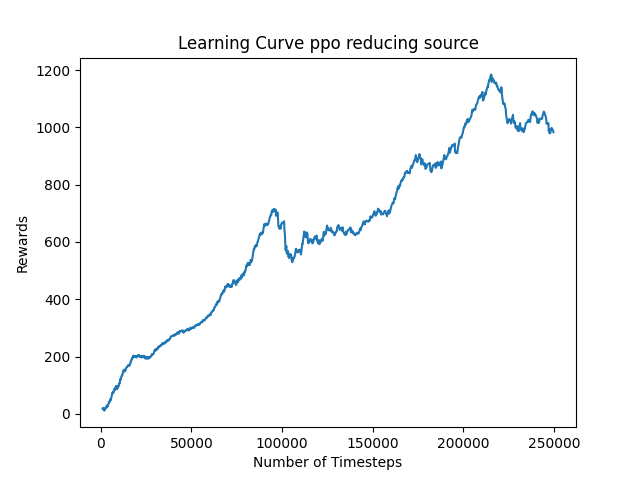
\includegraphics[width=\textwidth]{../images/Learning_curve_PPO_reducing_Source.png}
        \caption{PPO Source Domain with RRDR}
        \label{fig:ppo_source_rrdr}
    \end{minipage}
    \hfill
    \begin{minipage}{0.45\textwidth}
        \centering
        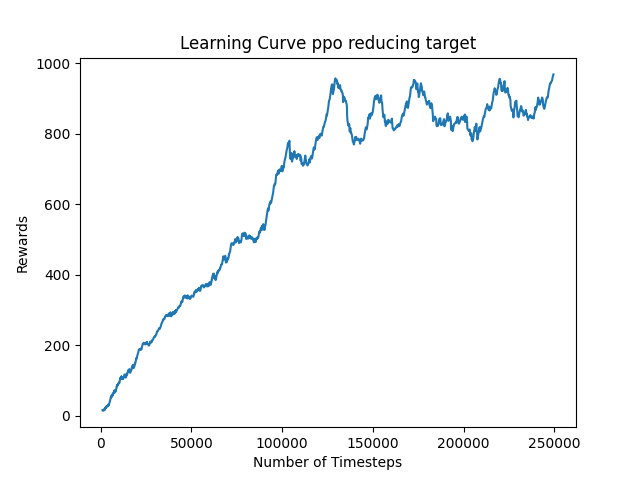
\includegraphics[width=\textwidth]{../images/Learning_curve_PPO_reducing_Target.png}
        \caption{PPO Target Domain with RRDR}
        \label{fig:ppo_target_rrdr}
    \end{minipage}

\end{figure}

In the following table, I report the mean reward and standard deviation obtained by the models trained with Reducing Ranged Domain Randomization in the source and target domains:

\begin{table}[H]
    \centering
    \begin{tabular}{|l|c|c|c|}
        \hline
        \textbf{Algorithm} & \textbf{Evaluation} & \textbf{Mean Reward} & \textbf{Standard Deviation} \\ \hline
        SAC & Source $\rightarrow$ Source & 1560.95 & 6.42 \\ 
        SAC & Source $\rightarrow$ Target & 1125.93 & 24.52 \\ 
        SAC & Target $\rightarrow$ Target & 637.40 & 29.50 \\ \hline
        PPO & Source $\rightarrow$ Source & 1524.11 & 76.85 \\ 
        PPO & Source $\rightarrow$ Target & 1376.73 & 247.33 \\ 
        PPO & Target $\rightarrow$ Target & 964.53 & 230.16 \\ \hline
    \end{tabular}
    \caption{Results of SAC and PPO with Reducing Ranged Domain Randomization.}
    \label{tab:results_rrdr}
\end{table}

The results show better results for both SAC and PPO considering the source to target evaluation obtained with UDR. This is obtained thanks to the nature of the implemented algorithm. The RRDR approach starts with large randomization ranges for body mass values, encouraging exploration of a wide variety of configurations in the early stages of training. This is particularly important because it allows the agent to experience diverse scenarios and adapt to a broader range of potential states. Over time, as the randomization factor is gradually reduced, the agent shifts from exploration to exploitation, focusing on optimizing its policy for more stable and predictable environments. This balance of exploration and exploitation helps the agent learn more robust policies that generalize better across domains.

However, even the results show that SAC and PPO achieve higher stabilities, the render results shows that both algorithms are not able to find a policy that moves correctly the hopper in both source and target domain. They achieve good results in the source to source evaluation, while in the source to target both algorithm fails. Statistically, I have found that SAC fails more than PPO considering the 100 episodes. A possible reason for this behaviour can be again related to the ranges. In this case, the increment of the ranges can be not enough to allow the SAC and PPO algorithm to learn a good policy in the target domain with a gradual increment. In previous tests, I have tested with linear decay, but performance for both algorithms was not good.

\subsection{Incremental Ranges Expansion Domain Randomization (IRE)}

The next set of experiments was conducted using the Incremental Ranges Expansion Domain Randomization (IRE) technique. The following four pictures shows the learning curve of SAC and PPO considering the source and the target domain with IRE.

\begin{figure}[H]
    \centering
    \begin{minipage}{0.45\textwidth}
        \centering
        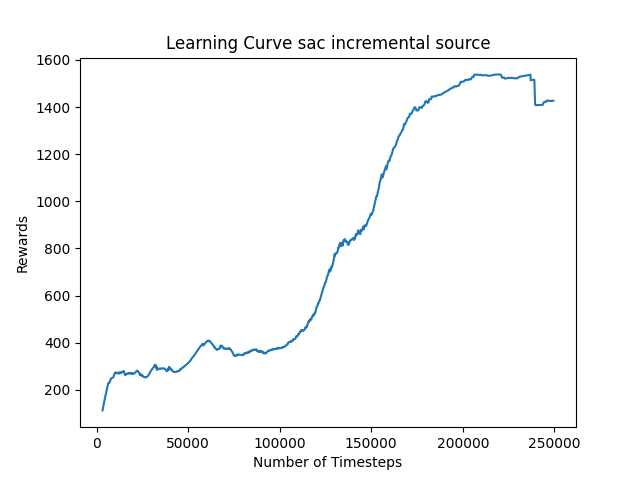
\includegraphics[width=\textwidth]{../images/Learning_Curve_SAC_Incremental_Source.png}
        \caption{SAC Source Domain with IRE}
        \label{fig:sac_source_ire}
    \end{minipage}
    \hfill
    \begin{minipage}{0.45\textwidth}
        \centering
        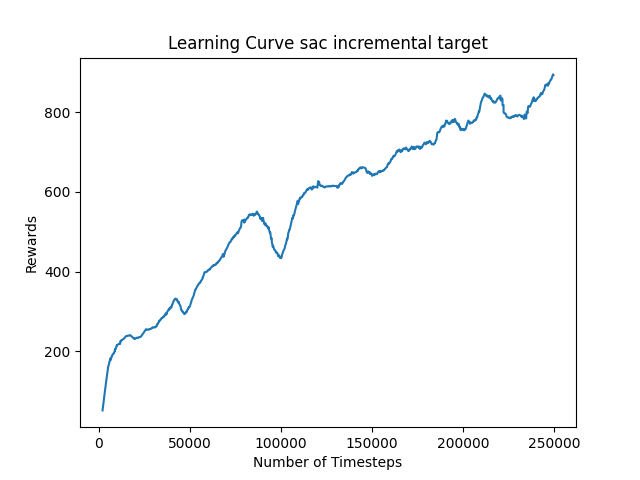
\includegraphics[width=\textwidth]{../images/Learning_Curve_SAC_Incremental_Target.png}
        \caption{SAC Target Domain with IRE}
        \label{fig:sac_target_ire}
    \end{minipage}
    \vfill
    \begin{minipage}{0.45\textwidth}
        \centering
        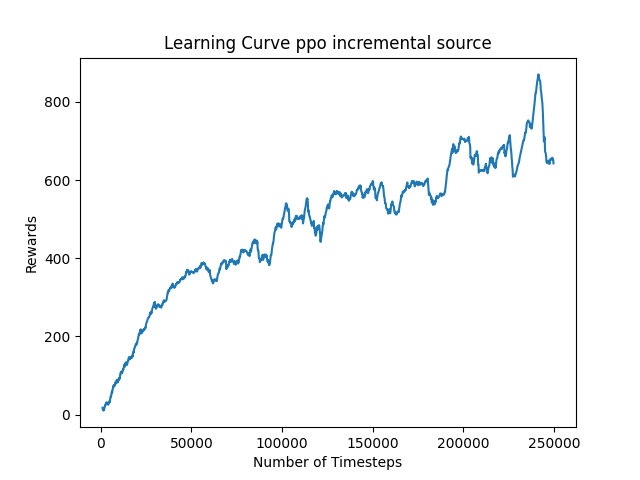
\includegraphics[width=\textwidth]{../images/Learning_Curve_PPO_Incremental_Source.png}
        \caption{PPO Source Domain with IRE}
        \label{fig:ppo_source_ire}
    \end{minipage}
    \hfill
    \begin{minipage}{0.45\textwidth}
        \centering
        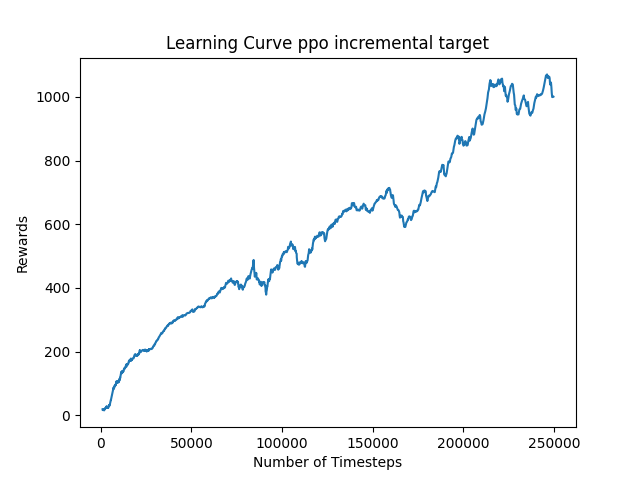
\includegraphics[width=\textwidth]{../images/Learning_Curve_PPO_Incremental_Target.png}
        \caption{PPO Target Domain with IRE}
        \label{fig:ppo_target_ire}
    \end{minipage}
\end{figure}

In the following table, I report the mean reward and standard deviation obtained by the models trained with Incremental Ranges Expansion Domain Randomization in the source and target domains:

\begin{table}[H]
    \centering
    \begin{tabular}{|l|c|c|c|}
        \hline
        \textbf{Algorithm} & \textbf{Evaluation} & \textbf{Mean Reward} & \textbf{Standard Deviation} \\ \hline
        SAC & Source $\rightarrow$ Source & 1555.75 & 44.13 \\ 
        SAC & Source $\rightarrow$ Target & 1079.24 & 99.46 \\ 
        SAC & Target $\rightarrow$ Target & 1041.11 & 334.47 \\ \hline
        PPO & Source $\rightarrow$ Source & 1196.54 & 294.40 \\ 
        PPO & Source $\rightarrow$ Target & 1031.03 & 89.09 \\ 
        PPO & Target $\rightarrow$ Target & 1383.46 & 189.42 \\ \hline
    \end{tabular}
    \caption{Results of SAC and PPO with Incremental Ranges Expansion Domain Randomization.}
    \label{tab:results_ire}
\end{table}

The results show that both SAC and PPO achieve an overall higher mean rewards in the three evaluations compared to the results obtained with UDR, but also with an increase of the standard deviation value. This is obtained as a consequence  nature of the implemented algorithm. The IRE approach provides a structured progression of exploration and exploitation phases, allowing the agent to adapt to different dynamics over the course of training. The initial focus on narrower ranges in the early stages of training helps the agent learn a stable policy that generalizes well to the source domain. As the ranges expand gradually, the agent is exposed to more diverse dynamics, improving its adaptability and robustness. By the end of training, the agent has experienced a wide range of conditions, enabling it to perform well in the target domain. This structured approach to domain randomization helps the agent balance exploration and exploitation, leading to more robust and generalizable policies.

The behavior observed here is similar to that of the Reducing Ranged Domain Randomization (RRDR) renderings, even though the results are better. In the source-to-target evaluation, the performance is lower compared to the results achieved with RRDR. This outcome can be attributed to the limited ranges, which are insufficient for the agent to learn an effective policy in the target domain. Further tests could explore the use of broader ranges and alternative reduction methods to address this limitation.

This three different type of approaches were designed to work together. While UDR generates a working policy for PPO, considering a low mean reward, the other two algorithms improve the mean reward value, but are not able to find a working policy. The next three approaches are different combinations of the previous three algorithms.

\subsection{Exploration Uniform Domain Randomization (EUDR)}

The next set of experiments was conducted using the Exploration Uniform Domain Randomization (EUDR) technique. The following four pictures shows the learning curve of SAC and PPO considering the source and the target domain with EUDR.

\begin{figure}[H]
    \centering
    \begin{minipage}{0.45\textwidth}
        \centering
        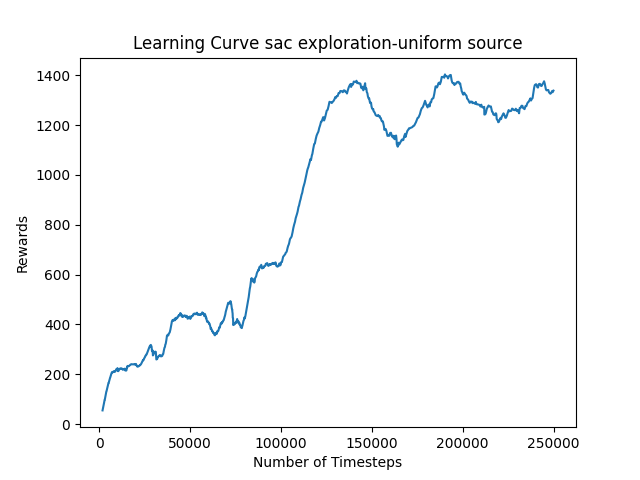
\includegraphics[width=\textwidth]{../images/Learning_Curve_SAC_EU_Source.png}
        \caption{SAC Source Domain with EUDR}
        \label{fig:sac_source_eudr}
    \end{minipage}
    \hfill
    \begin{minipage}{0.45\textwidth}
        \centering
        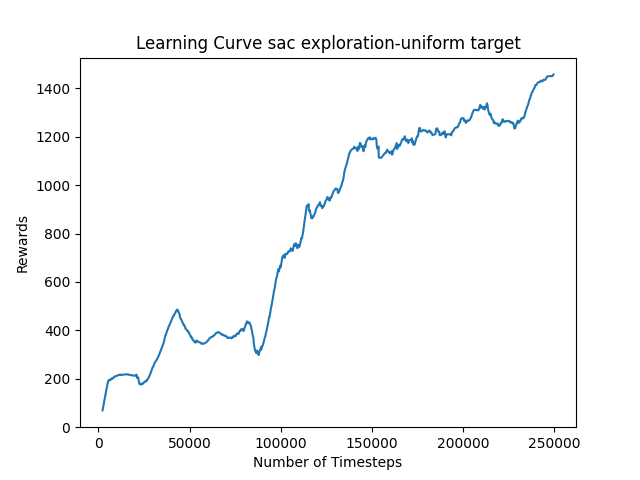
\includegraphics[width=\textwidth]{../images/Learning_Curve_SAC_EU_Target.png}
        \caption{SAC Target Domain with EUDR}
        \label{fig:sac_target_eudr}
    \end{minipage}
    \vfill
    \begin{minipage}{0.45\textwidth}
        \centering
        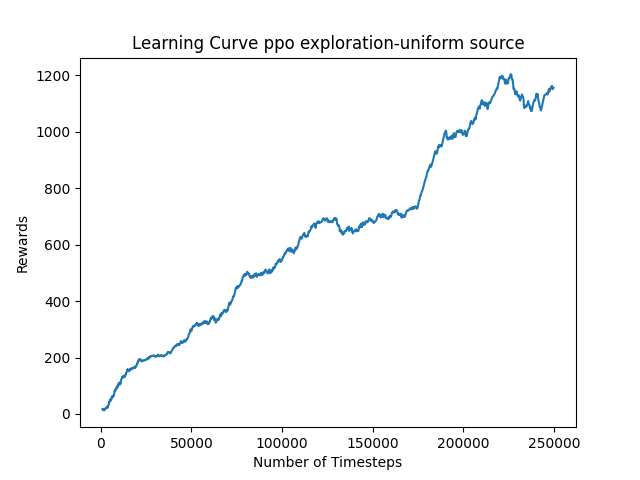
\includegraphics[width=\textwidth]{../images/Learning_Curve_PPO_EU_Source.png}
        \caption{PPO Source Domain with EUDR}
        \label{fig:ppo_source_eudr}
    \end{minipage}
    \hfill
    \begin{minipage}{0.45\textwidth}
        \centering
        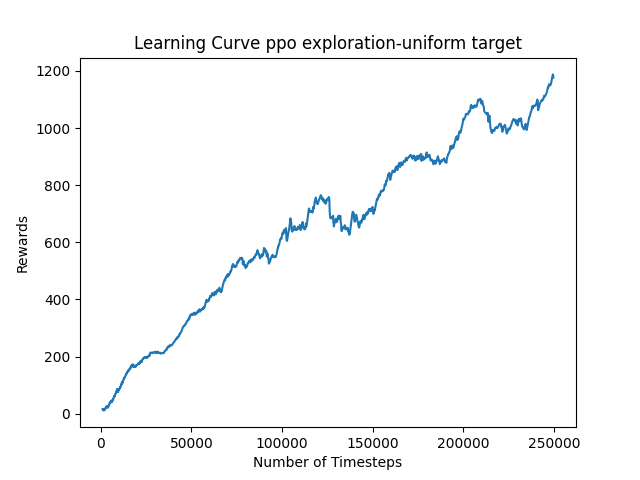
\includegraphics[width=\textwidth]{../images/Learning_Curve_PPO_EU_Target.png}
        \caption{PPO Target Domain with EUDR}
        \label{fig:ppo_target_eudr}
    \end{minipage}
\end{figure}

In the following table, I report the mean reward and standard deviation obtained by the models trained with Exploration Uniform Domain Randomization in the source and target domains:

\begin{table}[H]
    \centering
    \begin{tabular}{|l|c|c|c|}
        \hline
        \textbf{Algorithm} & \textbf{Evaluation} & \textbf{Mean Reward} & \textbf{Standard Deviation} \\ \hline
        SAC & Source $\rightarrow$ Source & 1368.33 & 191.46 \\ 
        SAC & Source $\rightarrow$ Target & 1108.02 & 152.44 \\ 
        SAC & Target $\rightarrow$ Target & 1540.32 & 1.60 \\ \hline
        PPO & Source $\rightarrow$ Source & 1403.84 & 1.73 \\ 
        PPO & Source $\rightarrow$ Target & 1482.32 & 5.62 \\ 
        PPO & Target $\rightarrow$ Target & 1493.53 & 34.60 \\ \hline
    \end{tabular}
    \caption{Results of SAC and PPO with Exploration Uniform Domain Randomization.}
    \label{tab:results_eudr}
\end{table}

The EUDR approach divides the training process into three distinct phases, each focusing on a specific goal: exploration, controlled randomization, and exploitation. The structured progression of phases allows the agent to adapt to different dynamics over the course of training, balancing exploration and exploitation. The initial exploration phase encourages the agent to explore a wide range of dynamics, while the controlled randomization phase narrows the focus to more stable environments. The exploitation phase further refines the policy for optimal performance. This structured approach helps the agent learn robust policies that generalize well across domains, improving adaptability and performance.

The results show different behaviours of the two models. While SAC reaches good mean reward values considering all the three evaluations, it sufferes of high standard deviation. The rendering show that it is not able to find a good policy that moves correctly the hopper. On the other hand, PPO reaches good mean reward values in all the three evaluations and more stable results. The rendering of these results shows a perfectly working hopper considering both the source environment and the target environment. 

The difference in behavior can be attributed to the nature of the two algorithms. SAC, as an off-policy algorithm, promotes extensive exploration but may struggle to efficiently exploit good solutions when faced with domain shifts (e.g., torso mass changes). This tendency can result in variability in performance and high standard deviation. During the increment phase of EUDR, SAC's broad exploration is amplified, potentially leading to instability early in training. Furthermore, SAC's reliance on a replay buffer means it samples from a diverse mix of transitions, which may include outdated or irrelevant experiences, hindering the development of a coherent policy suited to the target domain. Even as SAC progresses through the reducing and uniform phases, its off-policy nature and extensive exploration may prevent sufficient stabilization, resulting in fluctuating performance and persistently high standard deviation.

PPO, due to the fact that it is an on-policy algorithm, is more stable and efficient at exploiting good solutions. This allows it to learn a policy that generalizes well to the target domain, even with the exploration in the increment phase of the EUDR. PPO’s stability and efficiency in learning help it adapt to the target domain more effectively, leading to better performance and lower standard deviation. The structured progression of exploration and exploitation phases in the EUDR approach helps PPO balance exploration and exploitation, leading to more robust and generalizable policies.

\subsection{Dynamic Range Cycle Domain Randomization (DRC)}

The next set of experiments was conducted using the Dynamic Range Cycle Domain Randomization (DRC) technique. The following four pictures shows the learning curve of SAC and PPO considering the source and the target domain with DRC.

\begin{figure}[H]
    \centering
    \begin{minipage}{0.45\textwidth}
        \centering
        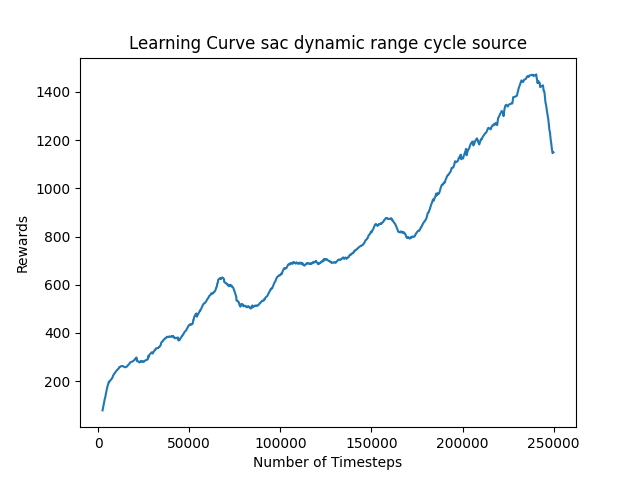
\includegraphics[width=\textwidth]{../images/Learning_Curve_SAC_DRC_Source.png}
        \caption{SAC Source Domain with DRC}
        \label{fig:sac_source_drc}
    \end{minipage}
    \hfill
    \begin{minipage}{0.45\textwidth}
        \centering
        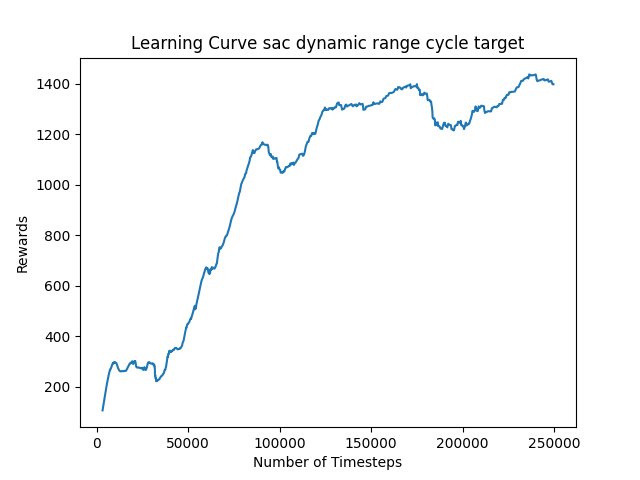
\includegraphics[width=\textwidth]{../images/Learning_Curve_SAC_DRC_Target.png}
        \caption{SAC Target Domain with DRC}
        \label{fig:sac_target_drc}
    \end{minipage}
    \vfill
    \begin{minipage}{0.45\textwidth}
        \centering
        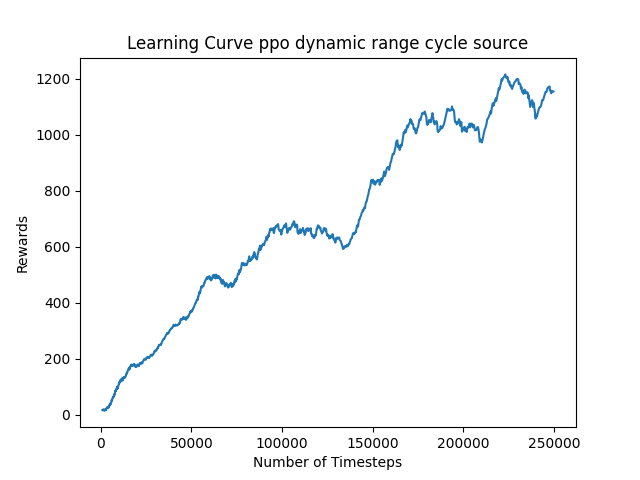
\includegraphics[width=\textwidth]{../images/Learning_Curve_PPO_DRC_Source.png}
        \caption{PPO Source Domain with DRC}
        \label{fig:ppo_source_drc}
    \end{minipage}
    \hfill
    \begin{minipage}{0.45\textwidth}
        \centering
        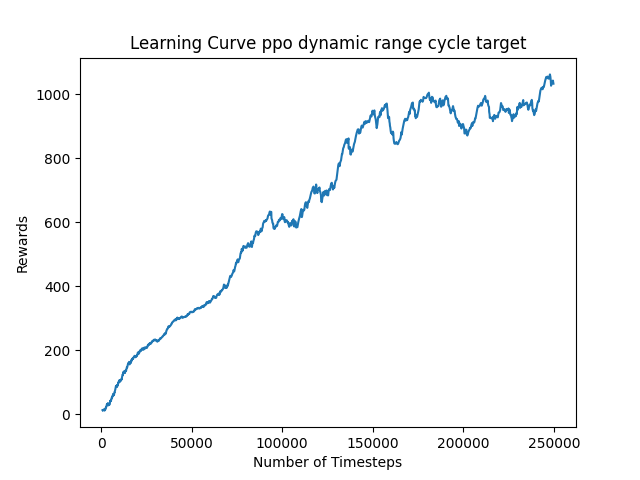
\includegraphics[width=\textwidth]{../images/Learning_Curve_PPO_DRC_Target.png}
        \caption{PPO Target Domain with DRC}
        \label{fig:ppo_target_drc}
    \end{minipage}
\end{figure}

In the following table, I report the mean reward and standard deviation obtained by the models trained with Dynamic Range Cycle Domain Randomization in the source and target domains:

\begin{table}[H]
    \centering
    \begin{tabular}{|l|c|c|c|}
        \hline
        \textbf{Algorithm} & \textbf{Evaluation} & \textbf{Mean Reward} & \textbf{Standard Deviation} \\ \hline
        SAC & Source $\rightarrow$ Source & 797.89 & 23.71 \\ 
        SAC & Source $\rightarrow$ Target & 616.59 & 10.04 \\ 
        SAC & Target $\rightarrow$ Target & 1497.44 & 1.57 \\ \hline
        PPO & Source $\rightarrow$ Source & 1532.42 & 17.32 \\ 
        PPO & Source $\rightarrow$ Target & 1519.38 & 181.27 \\ 
        PPO & Target $\rightarrow$ Target & 1580.80 & 37.97 \\ \hline
    \end{tabular}
    \caption{Results of SAC and PPO with Dynamic Range Cycle Domain Randomization.}
    \label{tab:results_drc}
\end{table}

This approach is different from the previous one. The DRC approach focuses on cycling through different ranges of randomization, allowing the agent to explore a wide variety of dynamics over the course of training. Starting with fixed ranges in the early stages of training, the agent learns a stable policy that generalizes well to the source domain. As the training progresses, the ranges expand to encourage exploration of more diverse environments. Then, the reduction of ranges helps the agent focus on more stable conditions, improving its adaptability and robustness. This cycling through different ranges helps the agent balance exploration and exploitation, leading to more robust and generalizable policies.

Also in this case, the results describe perfectly the behaviour that can be seen in the renderings. SAC is not able to find a good policy that moves correctly the hopper in both the source and the target domain, reaching the worst behaviour since now. All the tests episodes failed after two hopper steps. The mean reward values are lower compared to the results obtained with the other domain randomization techniques. On the other hand, PPO is able to find a good policy that moves correctly the hopper in both the source and the target domain. The mean reward values are higher compared to the results obtained with the other domain randomization techniques, but the high variance in the source to target environment is caused by few fails during the test episodes.

SAC is unable to adapt well to the dynamic changes introduced by the randomization phases, particularly during the uniform phase at the beginning, which may make it difficult for SAC to develop a meaningful policy due to the wide randomization ranges.
The high values assigned to the entropy coefficient in the increment phase and uniform phase likely encourage the agent to explore too broadly, without converging on a good solution. 

SAC struggles with Dynamic Range Cycle Domain Randomization due to its excessive exploration and inability to adapt effectively to the changing domain conditions. This leads to poor performance and high failure rates during test episodes.
PPO, on the other hand, benefits from its ability to gradually reduce exploration and exploit learned policies more effectively. This results in higher mean rewards and a better ability to generalize to both the source and target domains, despite occasional variability due to test failures.

\subsection{Dynamic Exploration Domain Randomization (DEDR)}

The next and last set of experiments was conducted using the Dynamic Exploration Domain Randomization (DEDR) technique. The following four pictures shows the learning curve of SAC and PPO considering the source and the target domain with DEDR.

\begin{figure}[H]
    \centering
    \begin{minipage}{0.45\textwidth}
        \centering
        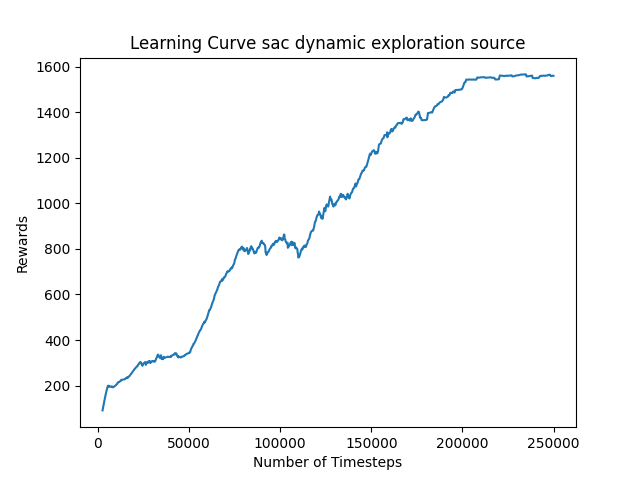
\includegraphics[width=\textwidth]{../images/Learning_Curve_SAC_DE_Source.png}
        \caption{SAC Source Domain with DEDR}
        \label{fig:sac_source_dedr}
    \end{minipage}
    \hfill
    \begin{minipage}{0.45\textwidth}
        \centering
        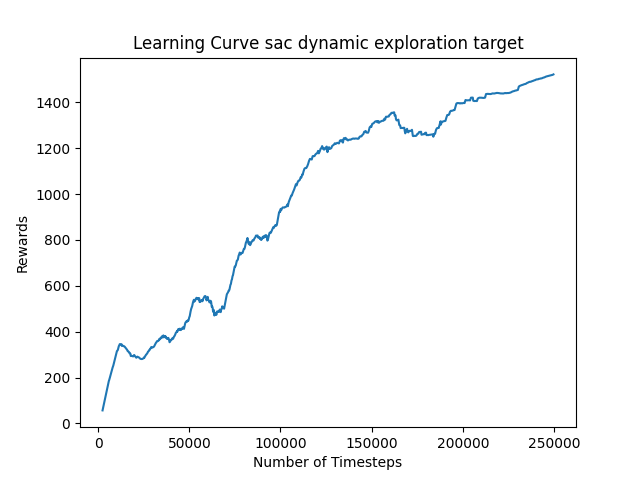
\includegraphics[width=\textwidth]{../images/Learning_Curve_SAC_DE_Target.png}
        \caption{SAC Target Domain with DEDR}
        \label{fig:sac_target_dedr}
    \end{minipage}
    \vfill
    \begin{minipage}{0.45\textwidth}
        \centering
        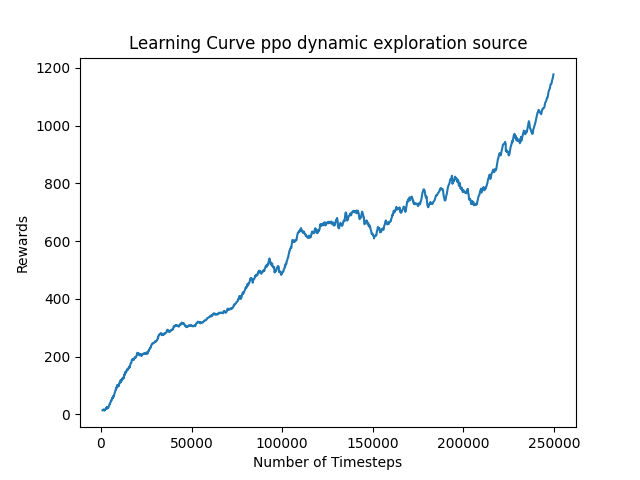
\includegraphics[width=\textwidth]{../images/Learning_Curve_PPO_DE_Source.png}
        \caption{PPO Source Domain with DEDR}
        \label{fig:ppo_source_dedr}
    \end{minipage}
    \hfill
    \begin{minipage}{0.45\textwidth}
        \centering
        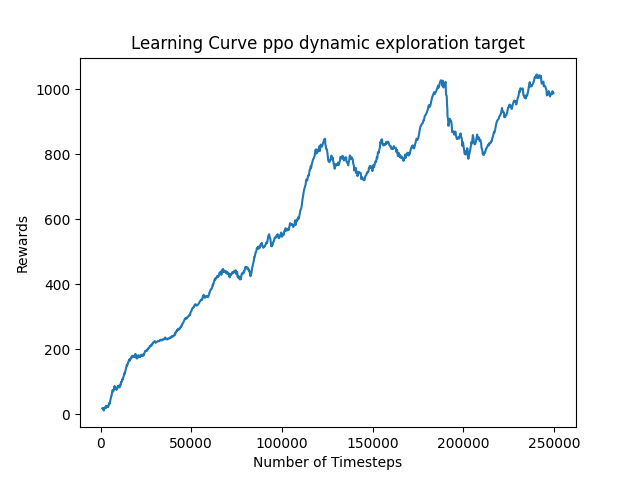
\includegraphics[width=\textwidth]{../images/Learning_Curve_PPO_DE_Target.png}
        \caption{PPO Target Domain with DEDR}
        \label{fig:ppo_target_dedr}
    \end{minipage}
\end{figure}

In the following table, I report the mean reward and standard deviation obtained by the models trained with Dynamic Exploration Domain Randomization in the source and target domains:

\begin{table}[H]
    \centering
    \begin{tabular}{|l|c|c|c|}
        \hline
        \textbf{Algorithm} & \textbf{Evaluation} & \textbf{Mean Reward} & \textbf{Standard Deviation} \\ \hline
        SAC & Source $\rightarrow$ Source & 1604.77 & 3.36 \\ 
        SAC & Source $\rightarrow$ Target & 1117.75 & 32.00 \\ 
        SAC & Target $\rightarrow$ Target & 1502.98 & 4.19 \\ \hline
        PPO & Source $\rightarrow$ Source & 1351.65 & 2.41 \\ 
        PPO & Source $\rightarrow$ Target & 1400.56 & 3.51 \\ 
        PPO & Target $\rightarrow$ Target & 1582.38 & 82.53 \\ \hline
    \end{tabular}
    \caption{Results of SAC and PPO with Dynamic Exploration Domain Randomization.}
    \label{tab:results_dedr}
\end{table}

The results shows an improvement in the performance for the SAC model. The combination of mean reward and standard deviation is the best considering all the other domain randomization techniques result. However, the rendering suggest that, also in this case, this model is not able to generalize the learned policy. While in the source to source rendering, the learned policy moves correctly the hopper, in the source to target rendering, the episode fails several time do to a wrong movement of the hopper. 
On the other end, PPO model reaches results very simular to the ones obtained in the EUDR algorithm. Also in this case, the movement of the hopper is perfect in the source to target rendering. 

SAC shows a significant improvement in the mean reward and standard deviation under DED-DR compared to previous methods. Although SAC still doesn't generalize as well as PPO, it demonstrates that a more dynamic exploration approach can improve policy stability and reward convergence, even if the generalization gap remains.

\section{Conclusion}

In this work, I have presented a comprehensive evaluation of different domain randomization techniques for training reinforcement learning agents in the Hopper environment. I have tested six different domain randomization techniques, including Uniform Domain Randomization (UDR), Reducing Ranged Domain Randomization (RRDR), Incremental Ranges Expansion Domain Randomization (IRE), Exploration Uniform Domain Randomization (EUDR), Dynamic Range Cycle Domain Randomization (DRC), and Dynamic Exploration Domain Randomization (DEDR). I have evaluated the performance of two reinforcement learning algorithms, Soft Actor-Critic (SAC) and Proximal Policy Optimization (PPO), in the source and target domains using these domain randomization techniques.

The results show that PPO outperforms SAC in terms of generalization across domains, achieving higher mean rewards and lower standard deviations in the target domain. PPO's stability and efficiency in learning allows it to adapt more effectively to changes in the environment, leading to better performance and robustness. SAC, on the other hand, struggles to generalize across domains due to its sensitivity to changes in the environment and limited exploration capabilities. The domain randomization techniques help improve the generalization capabilities of both algorithms, allowing them to adapt to different dynamics and environments.

Among the domain randomization techniques tested, EUDR and DEDR show the best results in terms of mean reward and standard deviation for both SAC and PPO. These techniques provide a structured progression of exploration and exploitation phases, allowing the agents to adapt to different dynamics over the course of training. The balanced approach to domain randomization helps the agents learn more robust policies that generalize well across domains, improving adaptability and performance.

The results obtained in this work provide valuable insights into the impact of domain randomization techniques on the generalization capabilities of reinforcement learning agents. By testing different domain randomization techniques and evaluating their performance in the source and target domains, we can gain a better understanding of how these techniques can improve the robustness and adaptability of reinforcement learning agents. These findings can help inform the development of more effective domain randomization techniques and improve the generalization capabilities of reinforcement learning agents in complex and dynamic environments.

\bibliographystyle{plainnat}
\begin{thebibliography}{9}
    \bibitem{Sutton2018}
    Richard S. Sutton and Andrew G. Barto,
    \textit{Reinforcement Learning: An introduction (Second Edition)},
    PDF.
    
    \bibitem{Kober2013}
    J. Kober, J. A. Bagnell, and J. Peters,
    \textit{Reinforcement learning in robotics: A survey},
    The International Journal of Robotics Research, 2013, PDF.
    
    \bibitem{Kormushev2013}
    P. Kormushev, S. Calinon, and D. G. Caldwell,
    \textit{Reinforcement learning in robotics: Applications and real-world challenges},
    2013, PDF.
    
    \bibitem{Hofer2020}
    S. Höfer, K. Bekris, A. Handa, J. C. Gamboa, F. Golemo, M. Mozifian, M. White,
    \textit{Perspectives on sim2real transfer for robotics: A summary of the R: SS 2020 workshop},
    2020, PDF.
    
    \bibitem{Tobin2017}
    J. Tobin, R. Fong, A. Ray, J. Schneider, W. Zaremba, and P. Abbeel,
    \textit{Domain Randomization for Transferring Deep Neural Networks from Simulation to the Real World},
    arXiv, Mar. 20, 2017, PDF.
    
    \bibitem{Peng2018}
    X. B. Peng, M. Andrychowicz, W. Zaremba, and P. Abbeel,
    \textit{Sim-to-real transfer of robotic control with dynamics randomization},
    2018, PDF.

    \bibitem{Haarnoja2018}
    T. Haarnoja, A. Zhou, P. Abbeel, and S. Levine,
    \textit{Soft Actor-Critic: Off-Policy Maximum Entropy Deep Reinforcement Learning with a Stochastic Actor},
    2018, PDF.

    \bibitem{Schulman2017}
    J. Schulman, F. Wolski, P. Dhariwal, A. Radford, and O. Klimov,
    \textit{Proximal policy optimization algorithms},
    2017, PDF.

    \bibitem{Akkaya2020}
    I. Akkaya, M. Andrychowicz, M. Chociej, M. Litwin, B. McGrew, A. Petron, A. Paino, M. Plappert, G. Powell, R. Ribas, J. Schneider, N. Tezak, J. Tworek, P. Welinder, L. Weng, Q. Yuan, W. Zaremba, L. Zhang,
    \textit{Solving Rubik’s Cube with a Robot Hand}, a preprint, 2020, PDF.


\end{thebibliography}


\end{document}